\documentclass[UTF8, a4paper, 11pt]{article}
\usepackage{diagbox}
\usepackage{subfigure}
\usepackage[UTF8, scheme=plain]{ctex}
\usepackage{fontspec}
\usepackage{float}
\usepackage{amsmath}
\newtheorem{myDef}{Definition}
\usepackage{graphicx}
\usepackage{geometry}
\usepackage{listings}
\usepackage{xcolor}
\usepackage{caption}
\geometry{scale=0.8}
\linespread{1.5}
\usepackage{hyperref}
\usepackage{color}
\usepackage{fontspec}
\usepackage{enumitem}
\usepackage[linesnumbered,boxed]{algorithm2e}    
\usepackage{xeCJK}
\usepackage{indentfirst} 
\usepackage{amssymb}
\graphicspath{{Pics/}} 	% 在于.tex同级的目录下创建名为pic的文件夹,存放图片


\setlength{\parindent}{2em}

\lstset{
    language={python},
    frame=shadowbox,
    breaklines=true,
    numbers=left,
    backgroundcolor=\color[RGB]{245,245,244},
    rulesepcolor=\color{red!20!green!20!blue!20},
    numberstyle={\color[RGB]{0,192,192}\tiny},
    basicstyle=\footnotesize \fontspec{Source Code Pro}
}
\setenumerate[1]{itemsep=0pt,partopsep=0pt,parsep=\parskip,topsep=0pt}
\setitemize[1]{itemsep=0pt,partopsep=0pt,parsep=\parskip,topsep=0pt}
\setdescription{itemsep=0pt,partopsep=0pt,parsep=\parskip,topsep=0pt}


\title{	
\normalfont \normalsize
\textsc{School of Data and Computer Science, Sun Yat-sen University} \\ [25pt] %textsc small capital letters
\rule{\textwidth}{0.5pt} \\[0.4cm] % Thin top horizontal rule
\huge 数电实验12\\ % The assignment title
\rule{\textwidth}{2pt} \\[0.5cm] % Thick bottom horizontal rule
\author{18308045 谷正阳}
\date{\normalsize\today}
}

\begin{document}
\maketitle
\tableofcontents
\newpage
\section{仿真实验}
\subsection{显示分秒}
\subsubsection{电路图}
\begin{figure}[H]
    \centering
    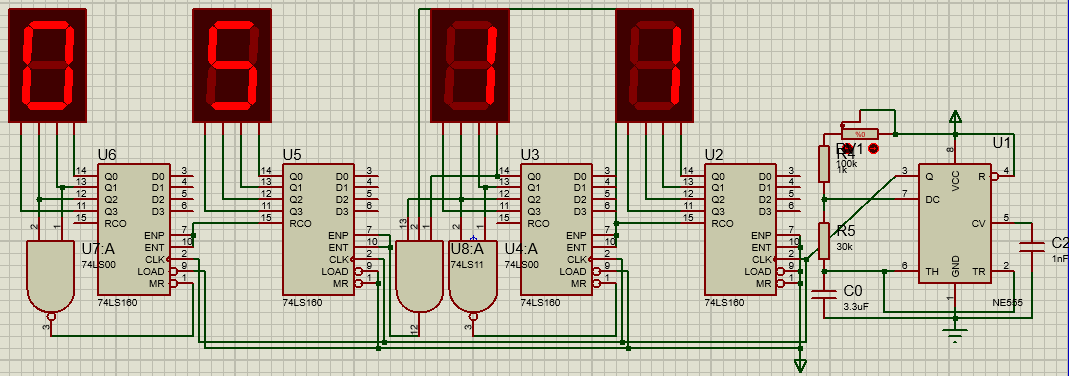
\includegraphics[width=0.8\textwidth]{ex12.1电路图.png}
\end{figure}
将555连成多谐振荡器,视作时钟,驱动两个由两个10分频连成60分频计数器。
\subsubsection{结果}
\href{run:./1.mp4}{点击查看演示视频1.mp4}
\section{实验箱实验}
\subsection{实验17}
\subsubsection{2}
\begin{figure}[H]
    \centering
    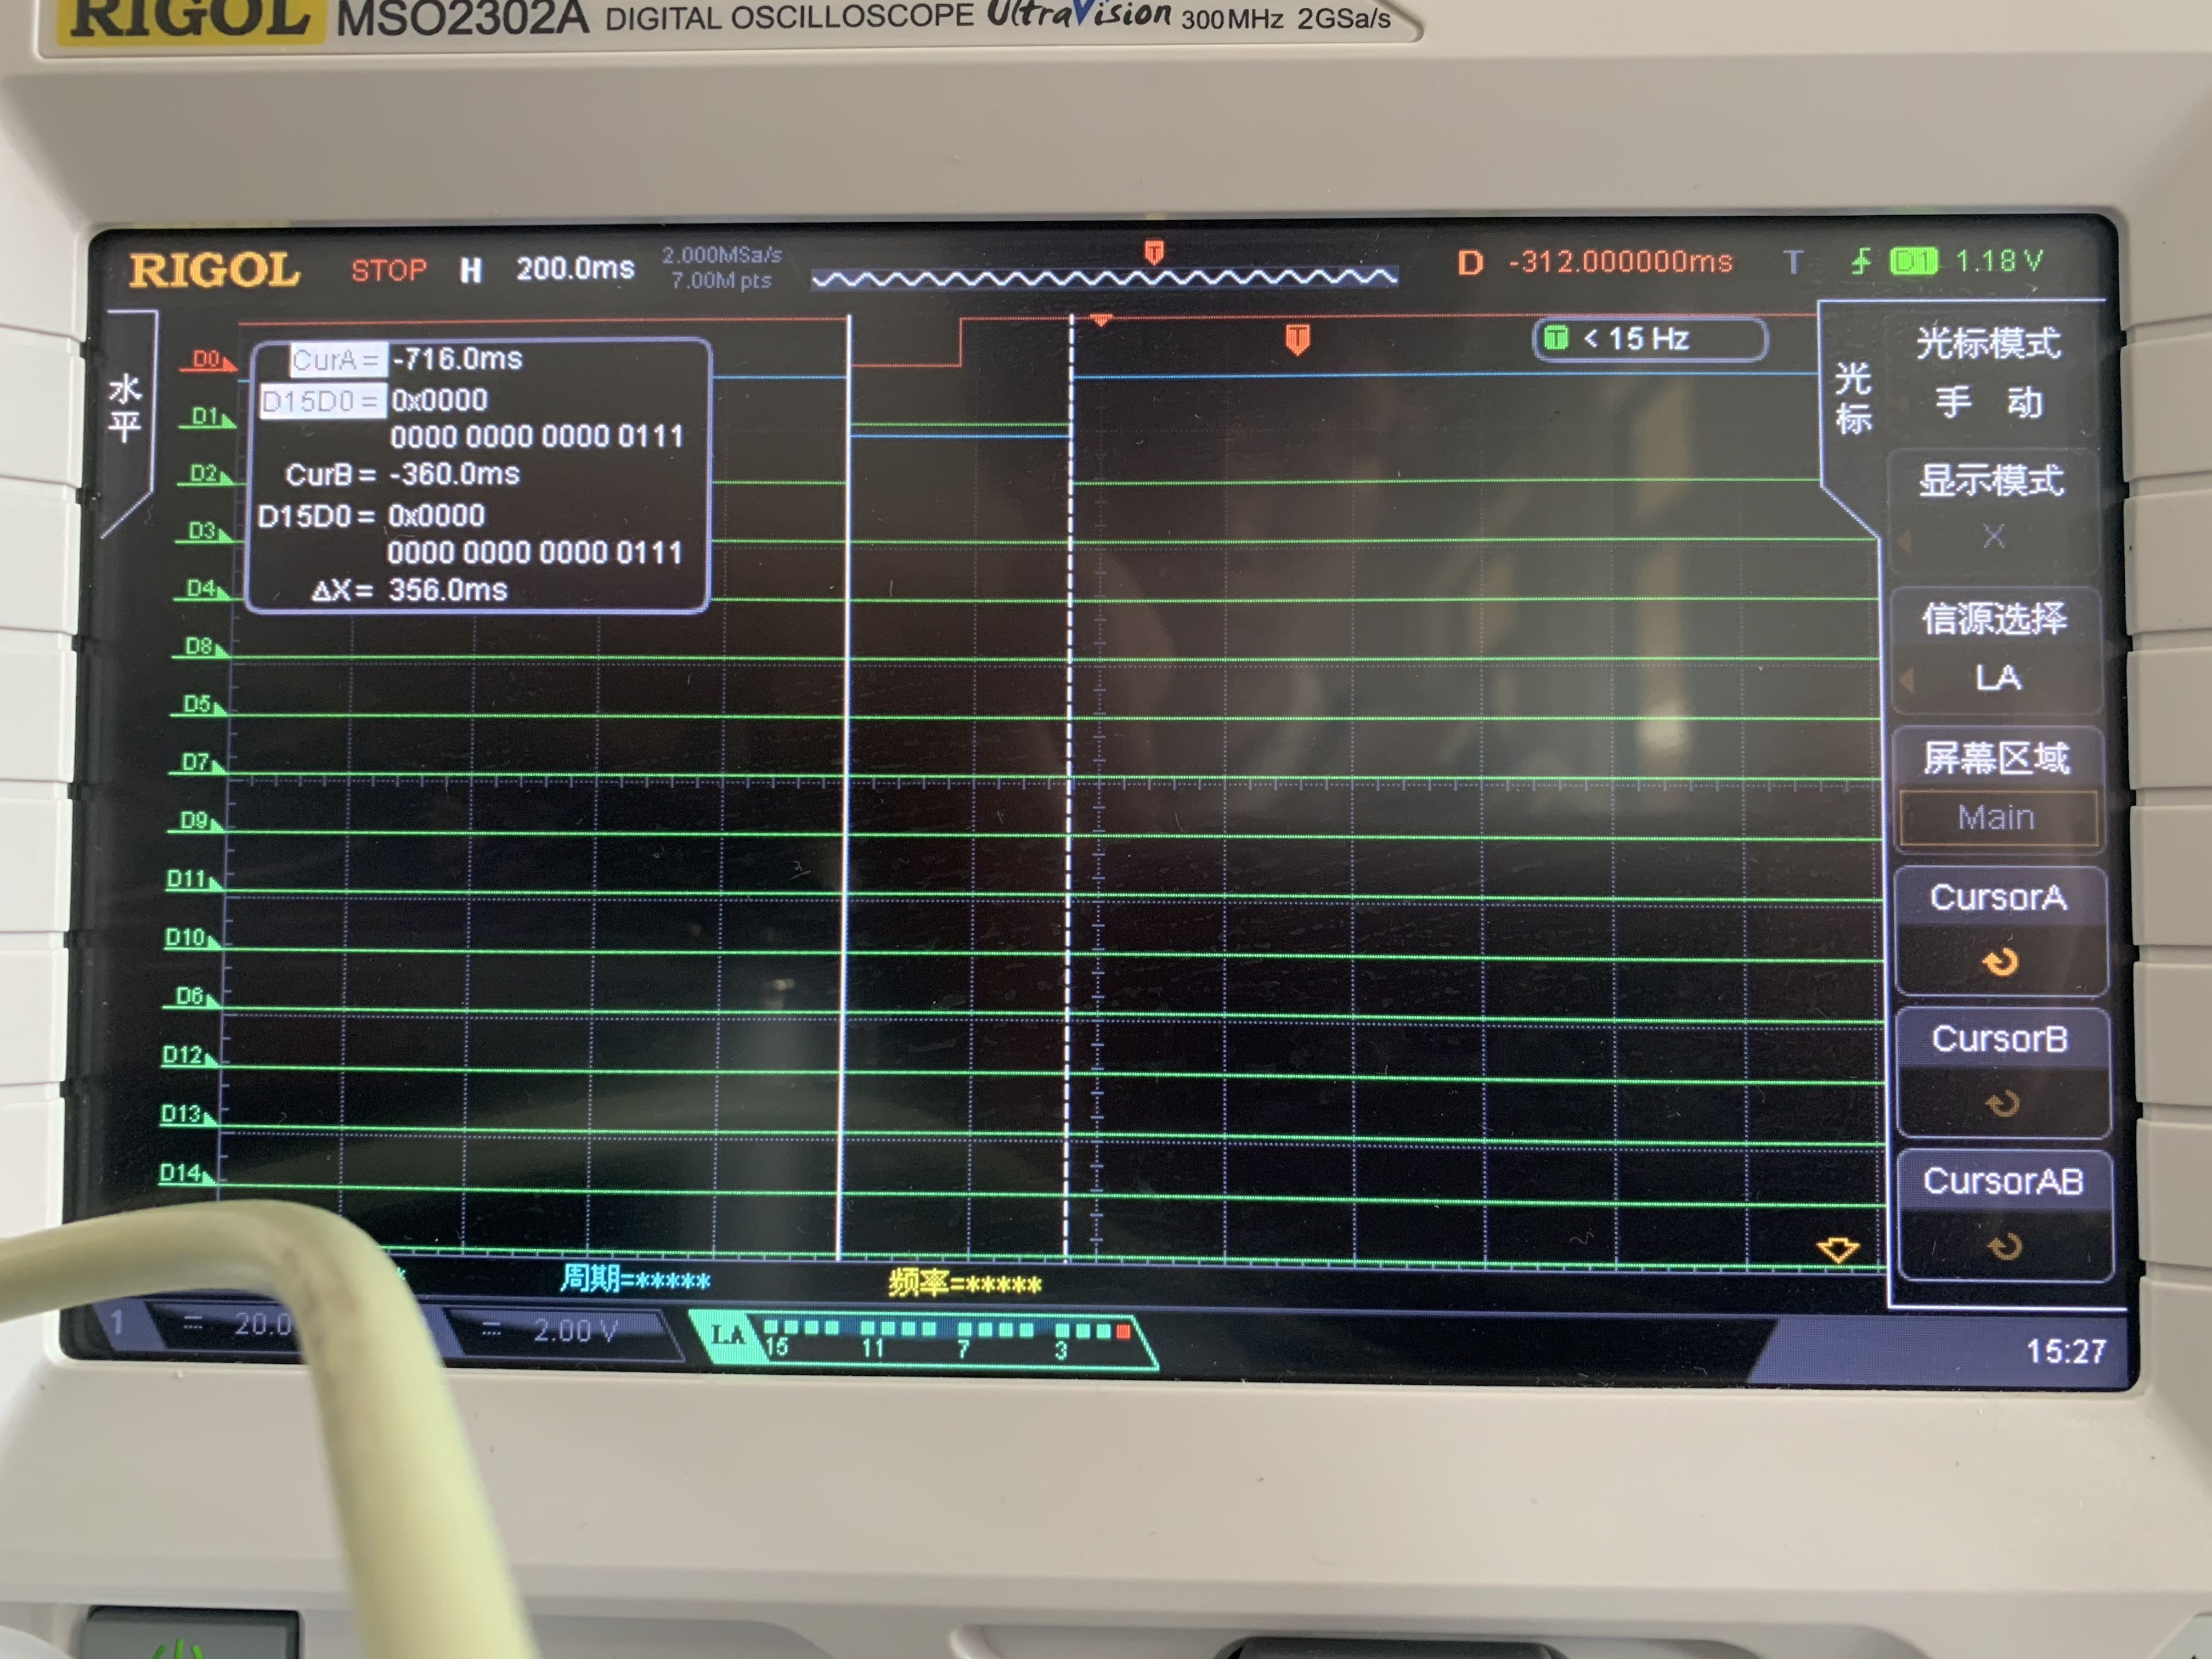
\includegraphics[width=0.8\textwidth]{1.png}
\end{figure}
首行输入,第二行基极,末行输出。
开始基极高电平,三极管导通,电流不流向电容,电容内无电荷。
输入一个负脉冲,基极低电平,三极管截止,电流流向电容,电容充电。
充电至$\frac23V_{CC}$,作用于比较器,最后影响基极输出高电平,三极管导通,电流不流向电容,电容放电,恢复到最开始的状态。
\begin{figure}[H]
    \centering
    
\includegraphics[width=0.8\textwidth]{2.png}
\end{figure}
增加电阻,可以看到脉宽由356ms变为436ms,因为正比于$R\cdot C$。
\subsubsection{3}
首行Vc1,次行Vc2,第三行基极,最后输出。
\begin{figure}[H]
    \centering
    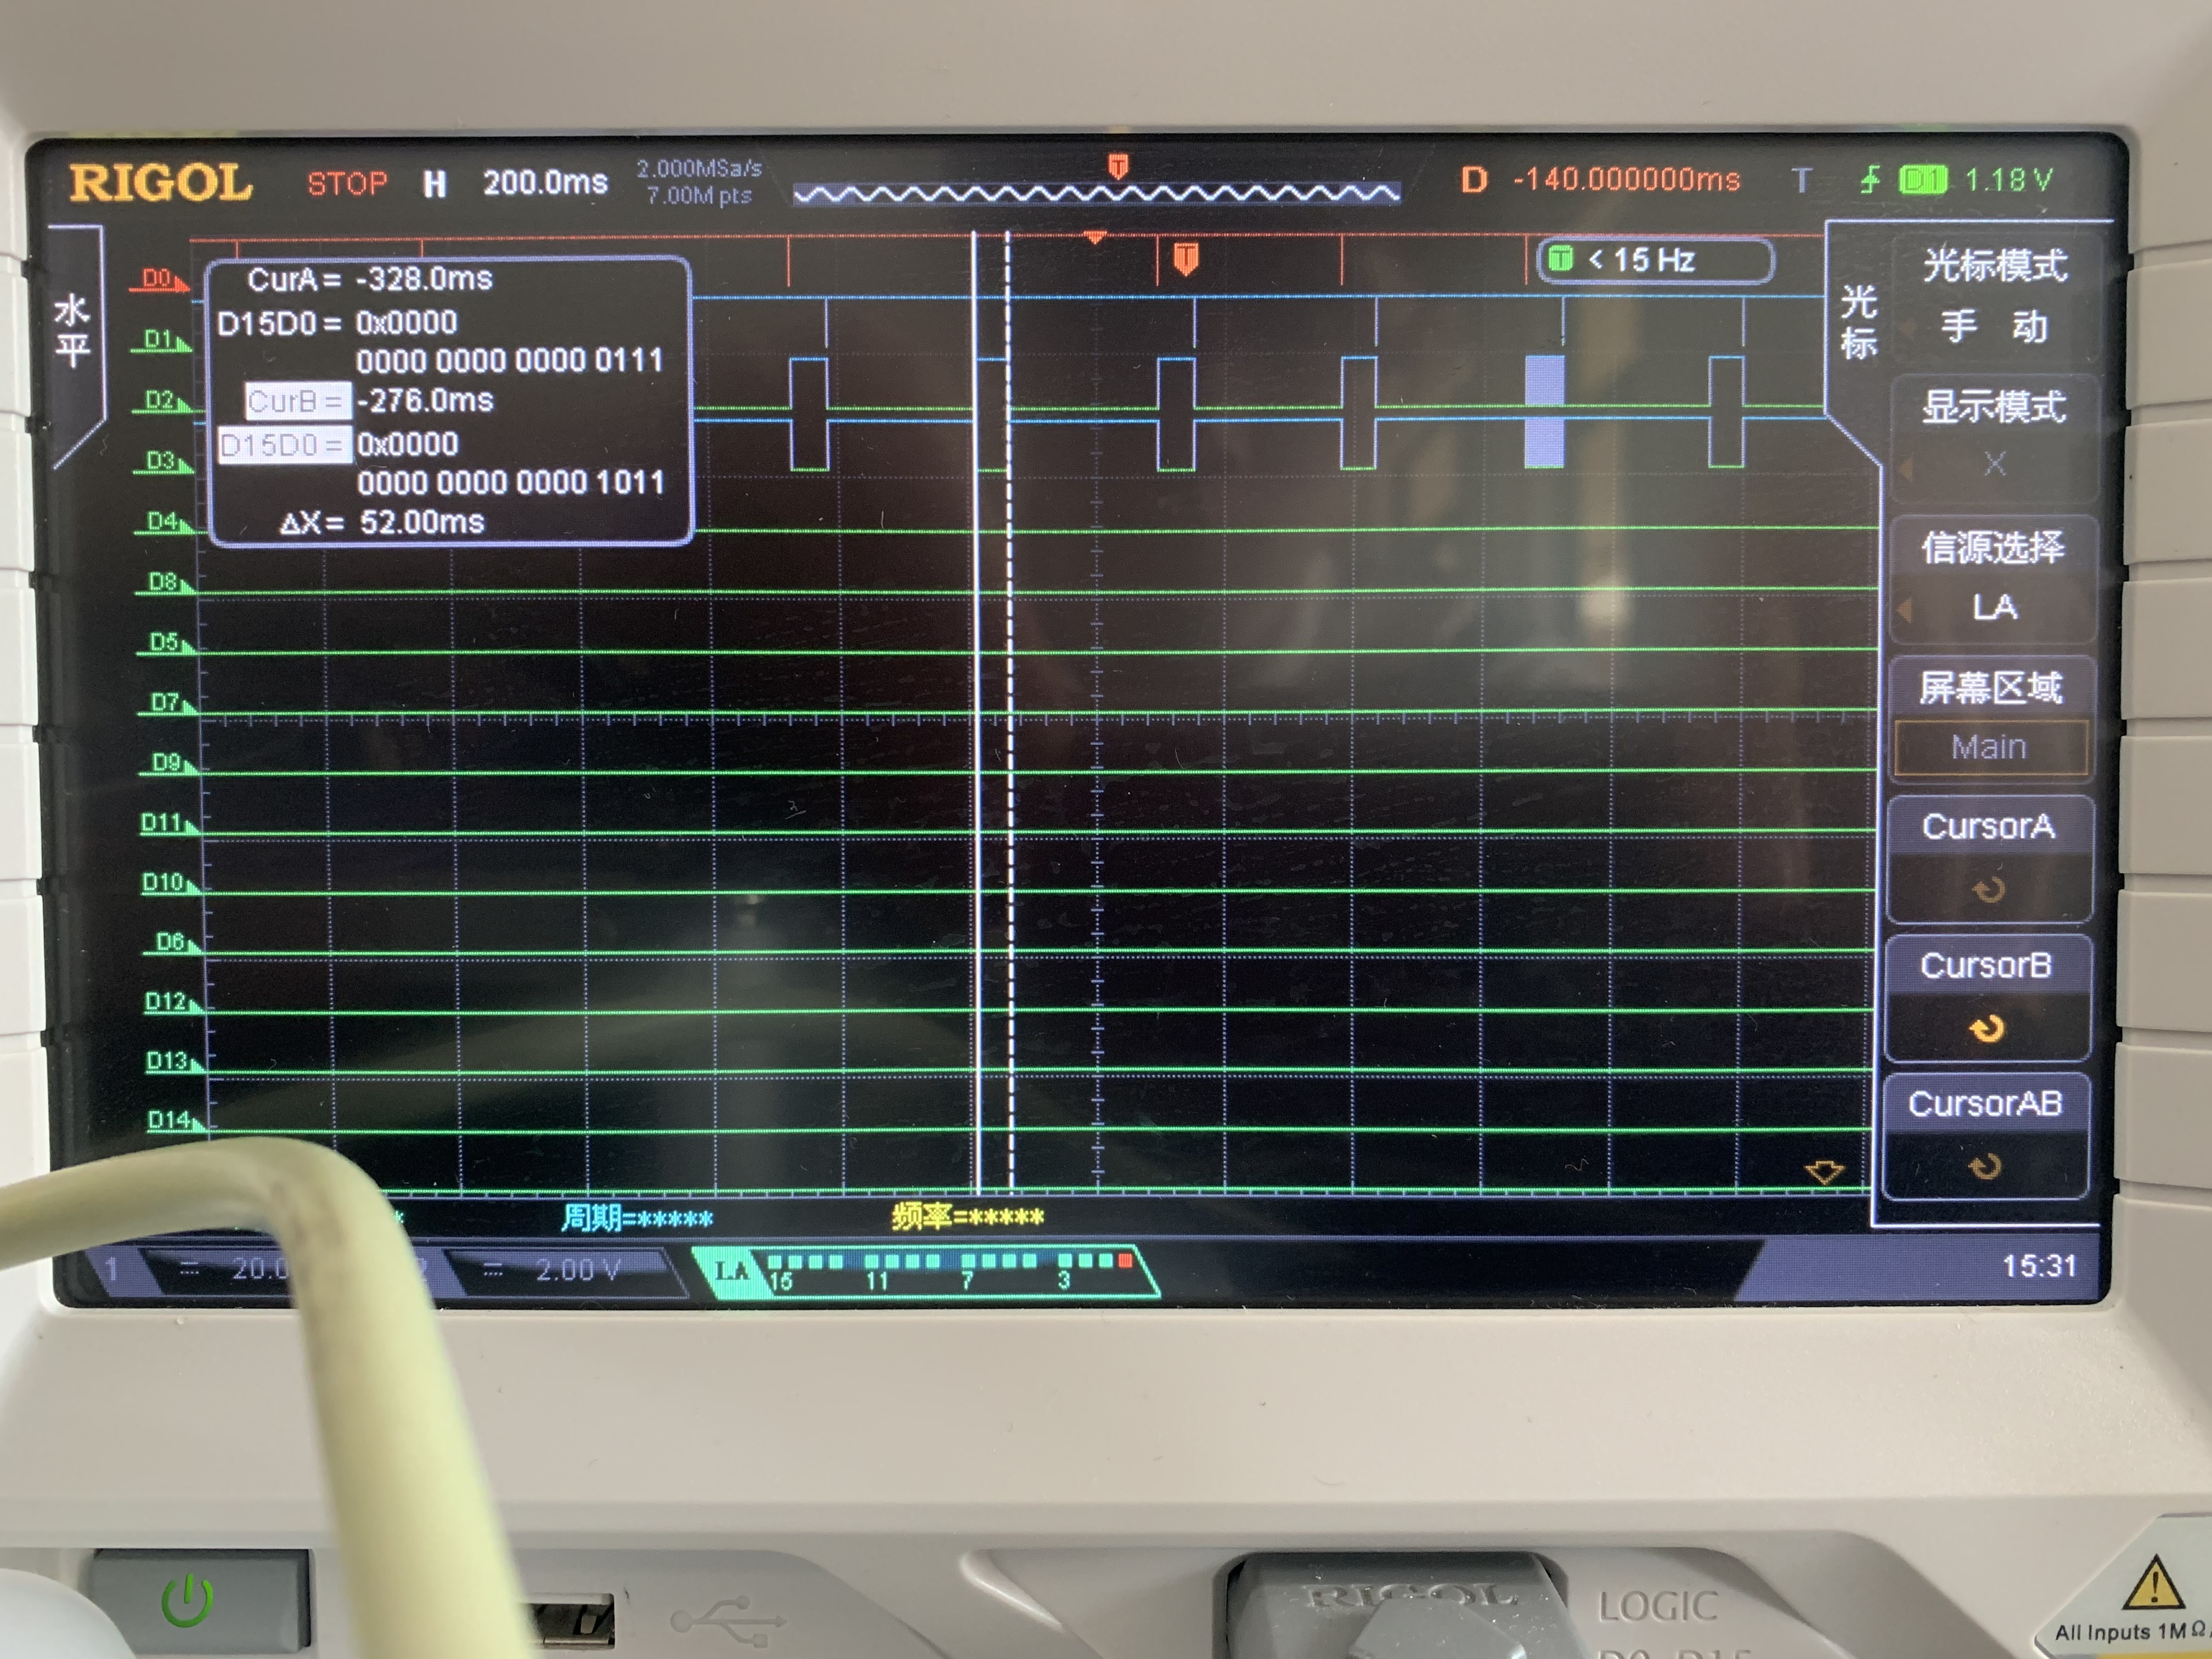
\includegraphics[width=0.8\textwidth]{3.png}
\end{figure}
\begin{figure}[H]
    \centering
    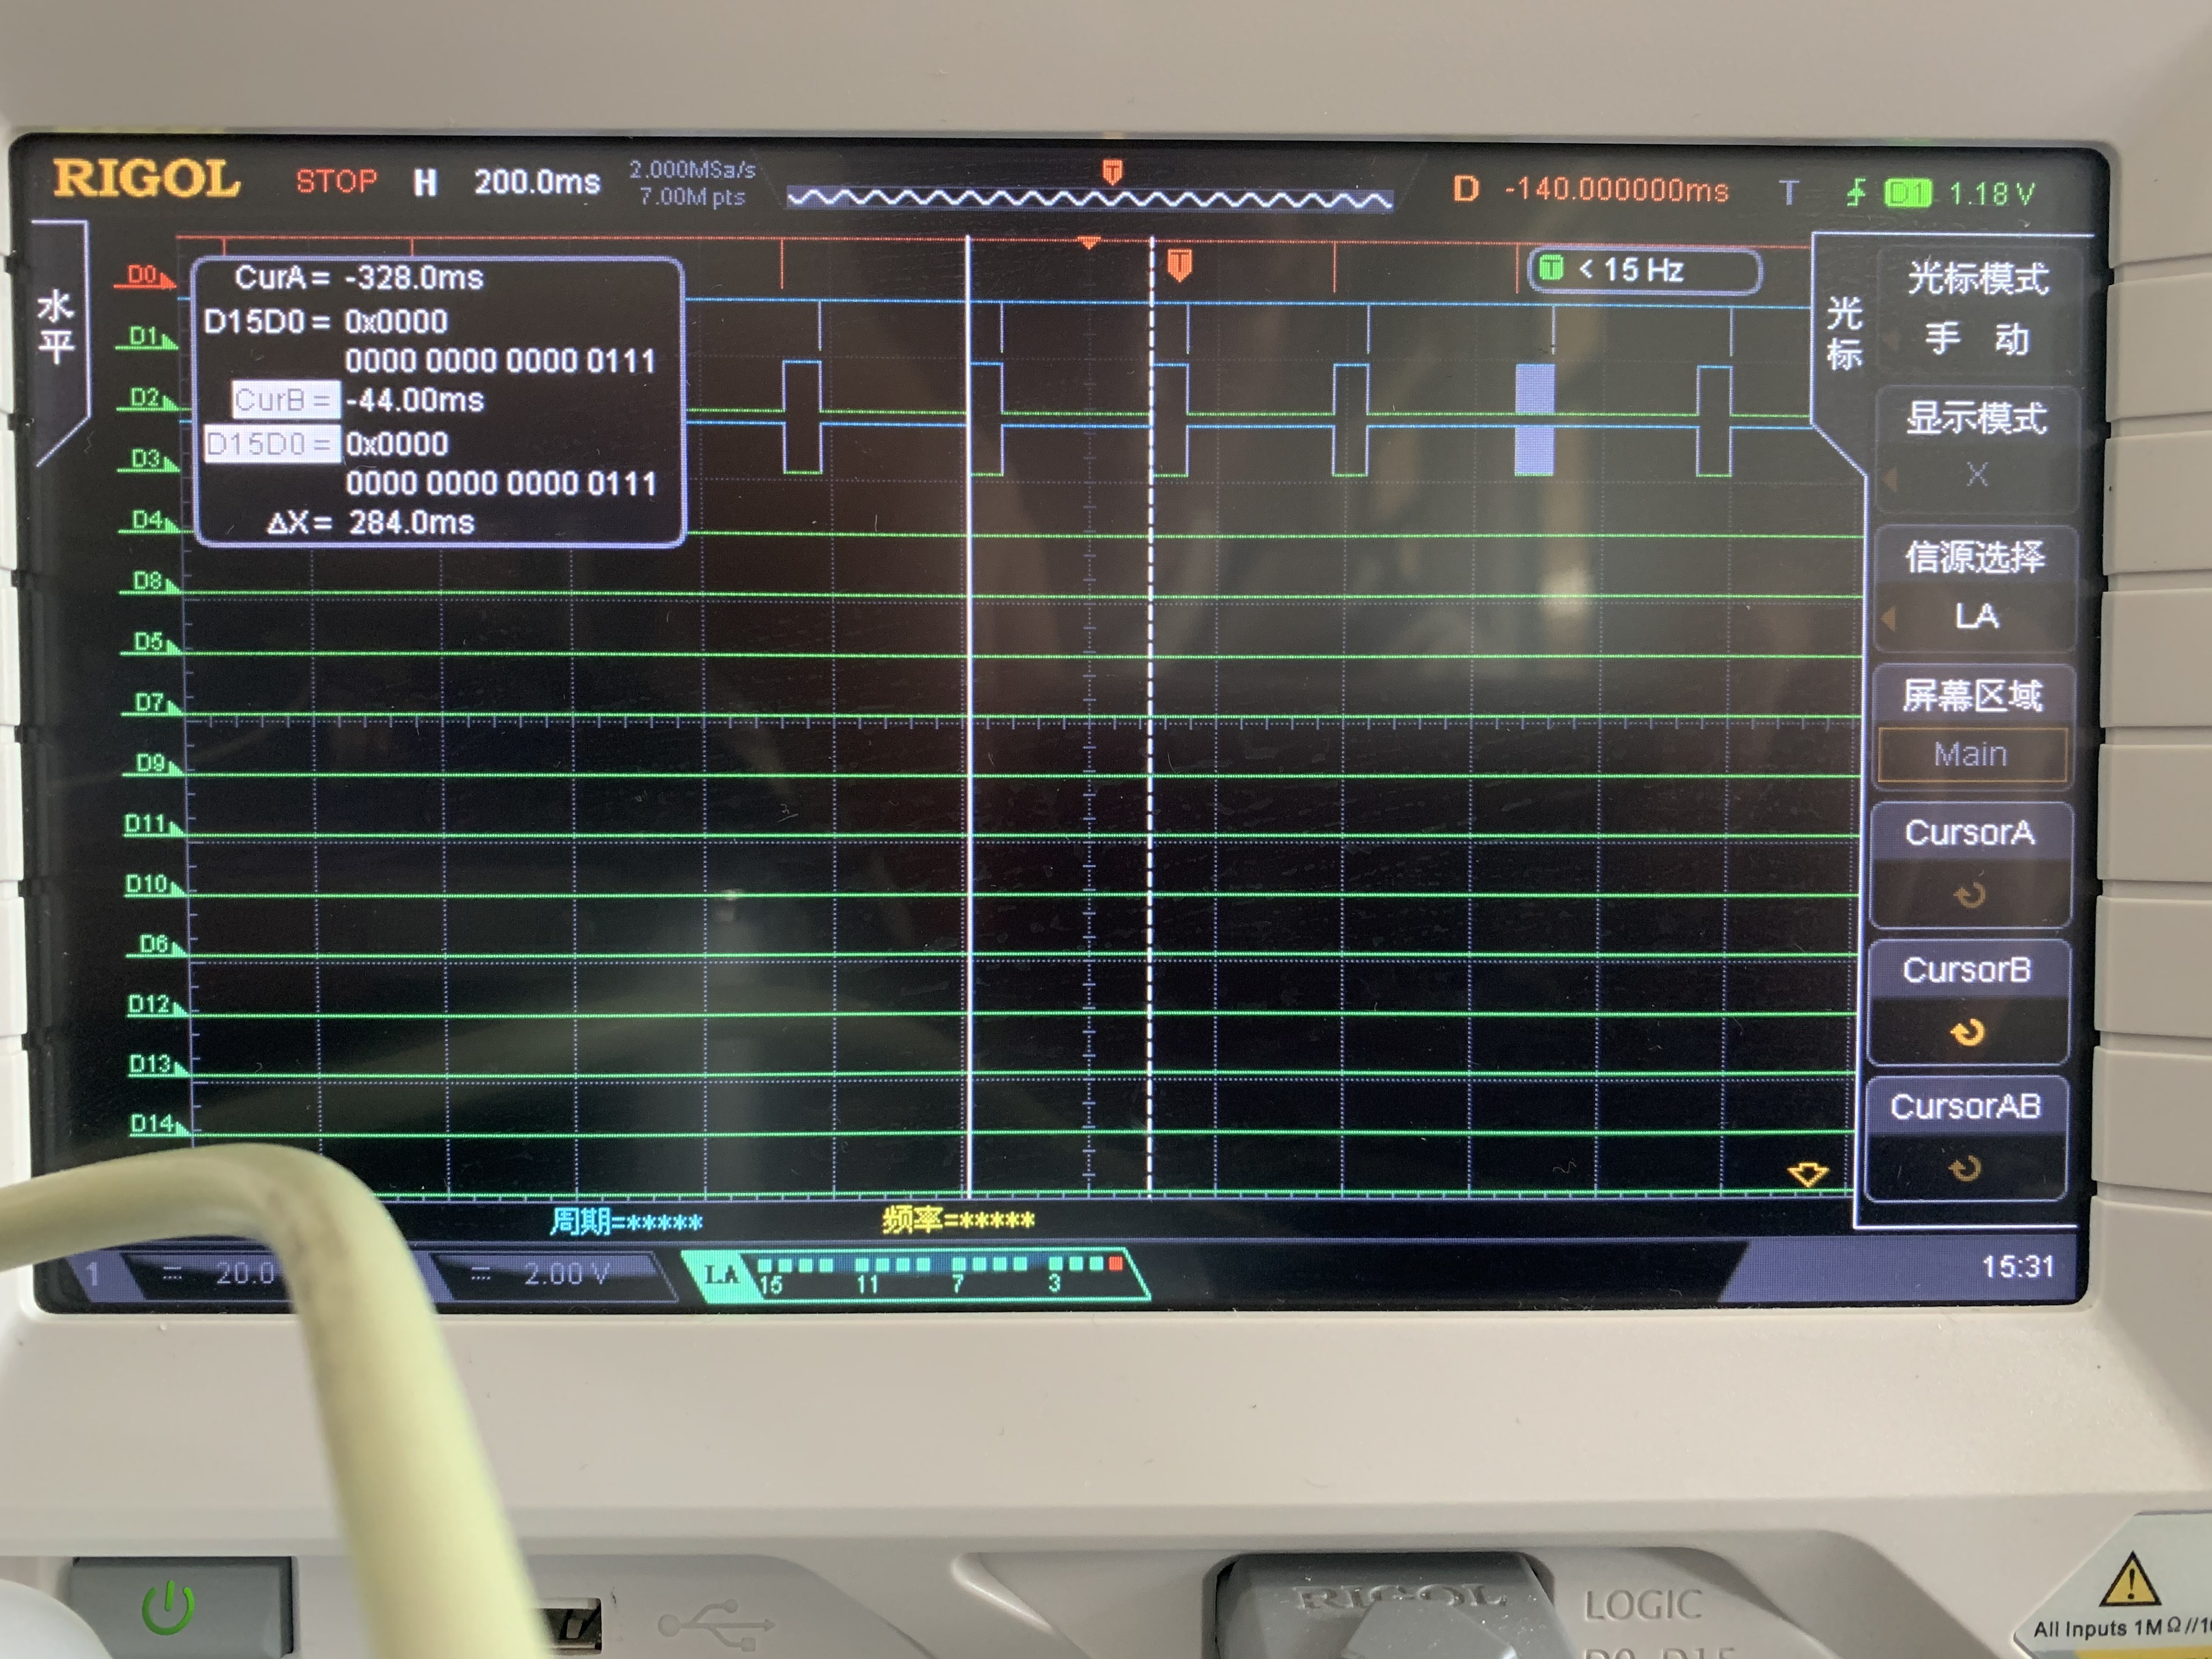
\includegraphics[width=0.8\textwidth]{4.png}
\end{figure}
初始C未充电,$V_{C1}$为1,$V_{C2}$为0,锁存器输出1,取反0给基极,三极管截断,电流导向电容,电容开始充电。
充至超过$\frac13V_{CC}$,$V_{C1},V_{C2}$都为1,锁存器保持1。
充至超过$\frac23V_{CC}$,$V_{C1}$为0,$V_{C2}$为1,锁存器输出0,取反1给基极,三极管导通,电流流向地,电容开始放电。
放了后,$V_{C1},V_{C2}$都为1,锁存器保持0。
放至低于$\frac13V_{CC}$,$V_{C1}$为1,$V_{C2}$为0,和最开始一样的状态。
\begin{figure}[H]
    \centering
    
\includegraphics[width=0.8\textwidth]{5.png}
\end{figure}
\begin{figure}[H]
    \centering
    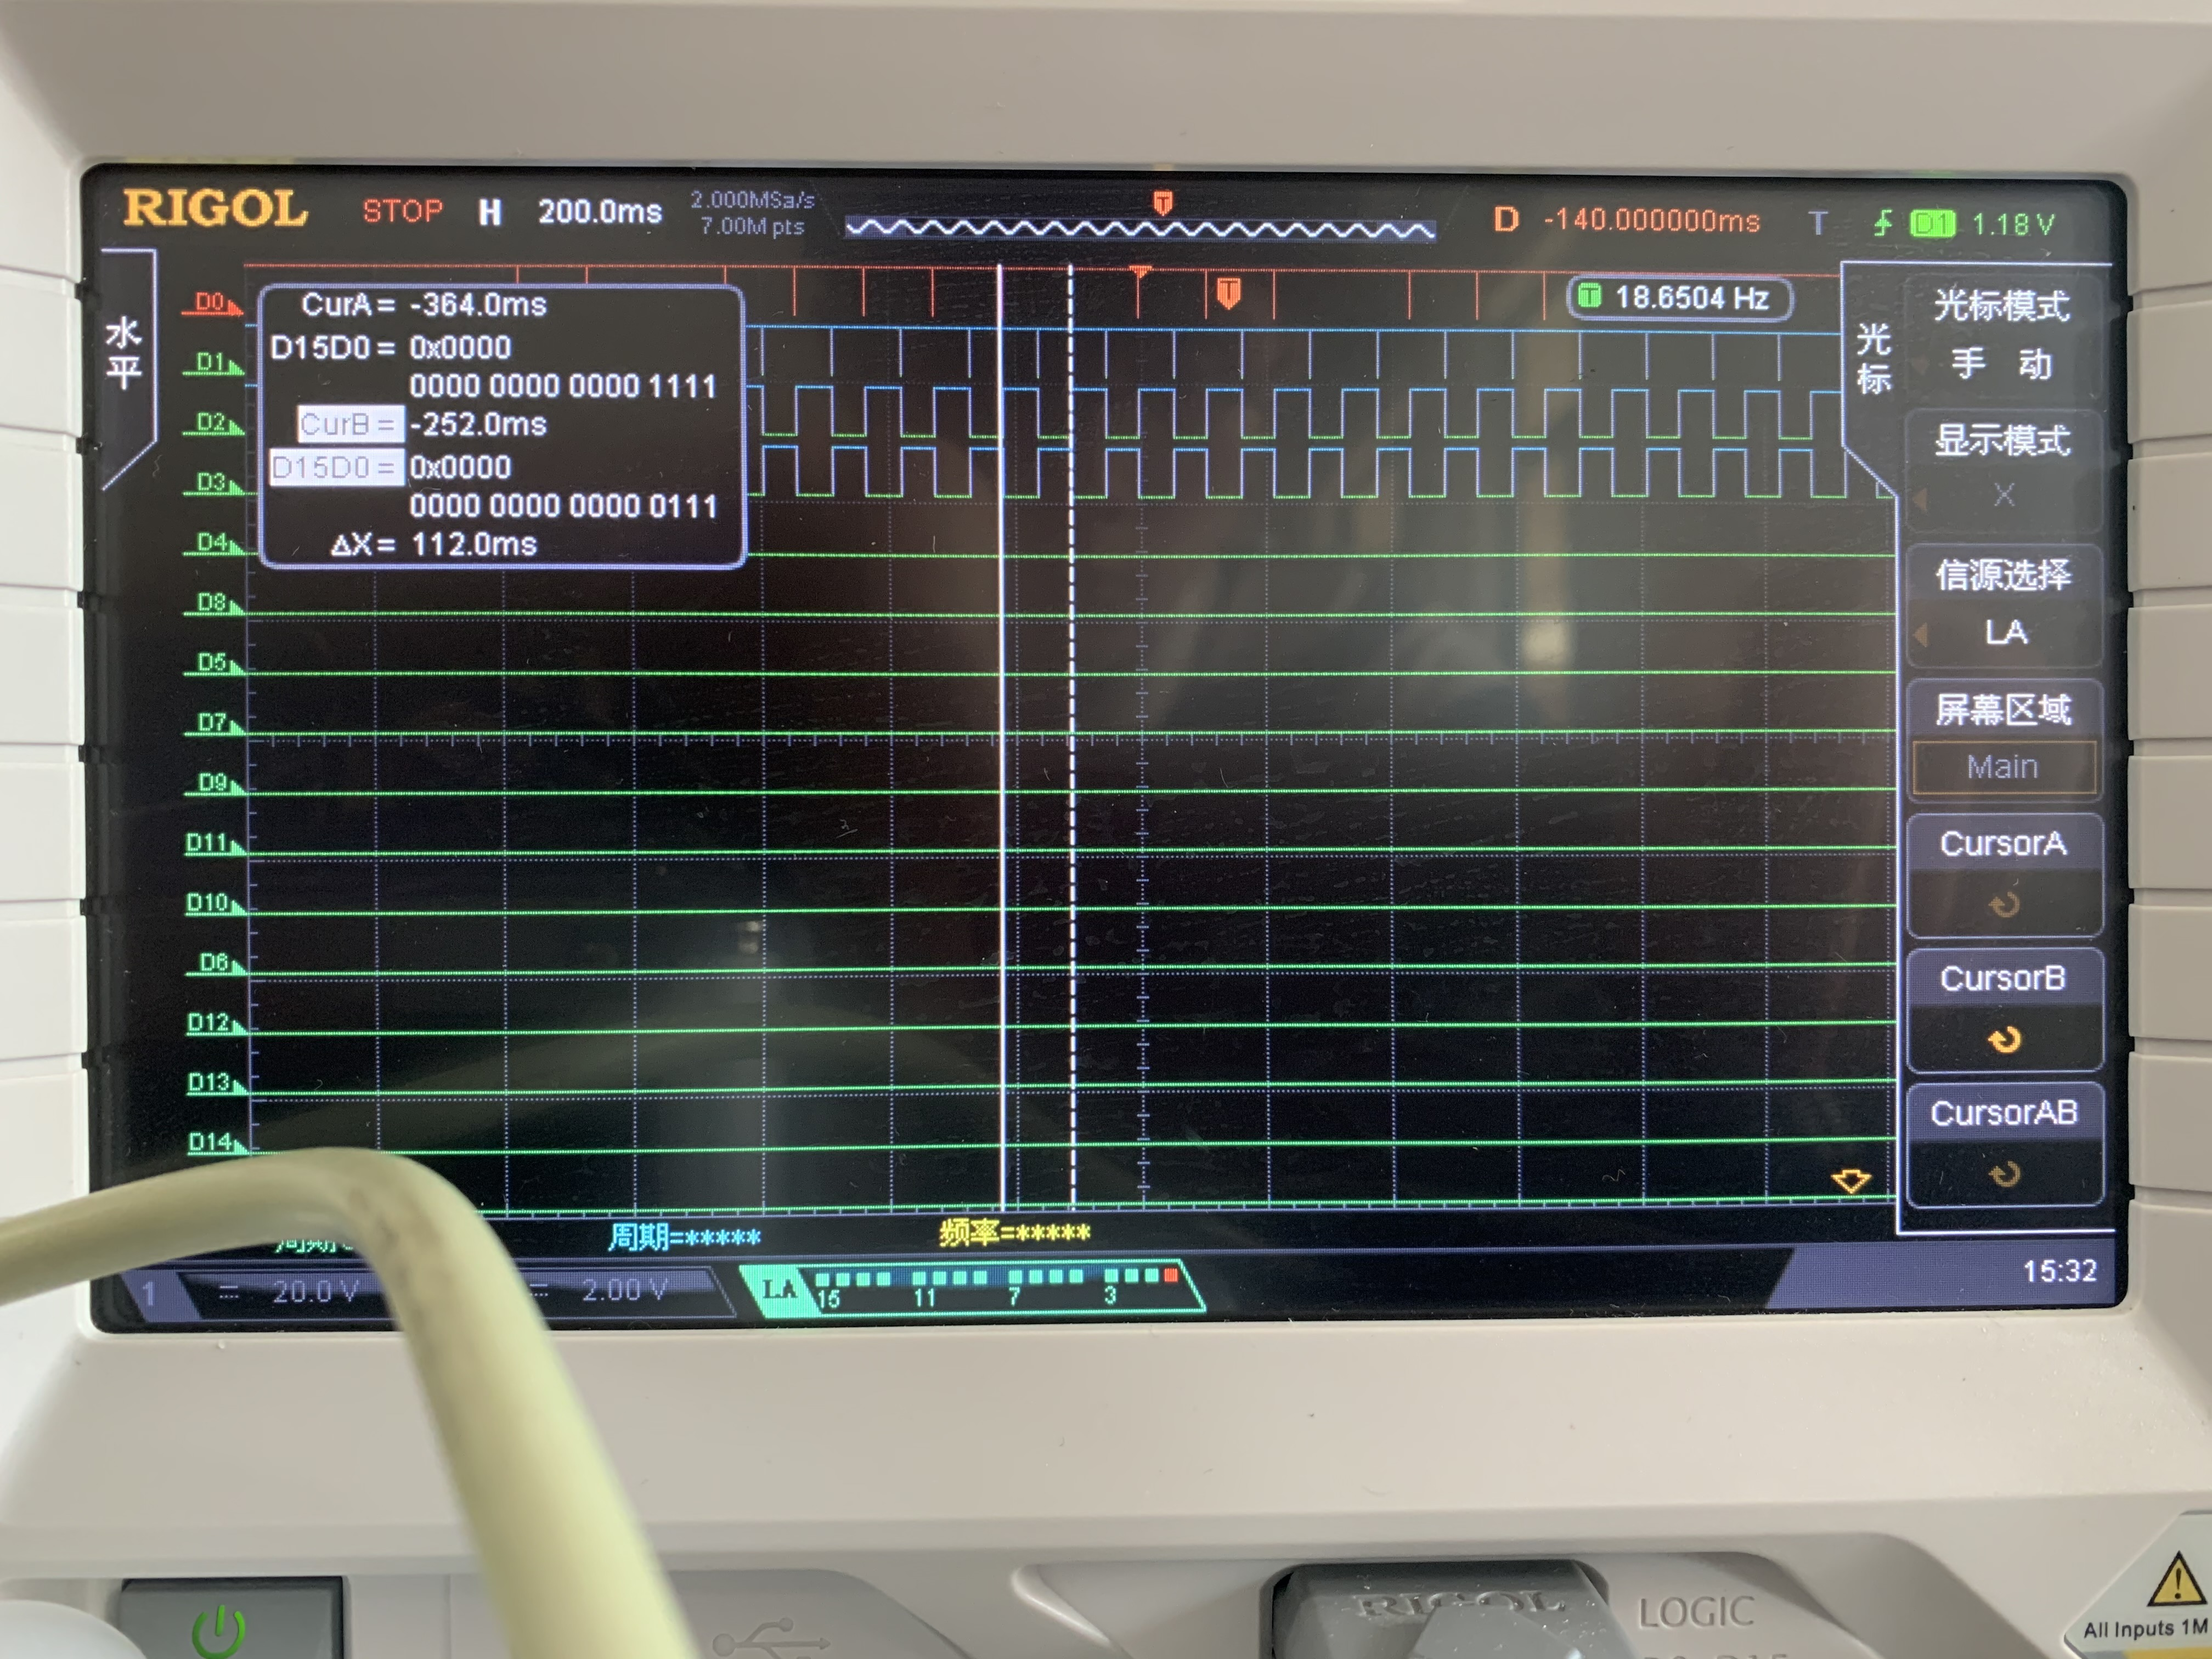
\includegraphics[width=0.8\textwidth]{6.png}
\end{figure}
占空的时间实际上是充电的时间,减小电阻,占空比由$\frac{284-52}{284}$减为$\frac{112-54}{112}$。
%\clearpage
%\bibliography{E:/Papers/LiuLab}
%\bibliographystyle{apalike}
\end{document}
%%% Local Variables:
%%% mode: latex
%%% TeX-master: t
%%% End:
